
%(BEGIN_QUESTION)
% Copyright 2014, Tony R. Kuphaldt, released under the Creative Commons Attribution License (v 1.0)
% This means you may do almost anything with this work of mine, so long as you give me proper credit

Sketch the necessary wire connections to create a three-phase transformer bank fulfilling the phasor diagrams shown to the left of the transformers:

$$\includegraphics[width=15.5cm]{i00848x01.eps}$$

Also, write the phase sequences (phase rotations) for both 3-phase busses, and identify whether the lower bus {\it leads}, {\it lags}, or is {\it in-phase} with the upper bus.

\underbar{file i00848}
%(END_QUESTION)





%(BEGIN_ANSWER)

This is not the only solution, but it will work.  Note the dots and numbers placed on the phasor diagrams to keep track of which transformers and which polarities are used:

$$\includegraphics[width=15.5cm]{i00848x02.eps}$$

The upper bus phase rotation is ABC.

\vskip 10pt

The lower bus phase rotation is ZYX.

\vskip 10pt

The phase shift between the two busses (comparing $V_A$ with $V_X$) is 90$^{o}$, with the lower bus {\it leading ahead of} the upper bus: $V_A = \angle -150^o$ and $V_X = \angle -60^o$

%(END_ANSWER)





%(BEGIN_NOTES)


%INDEX% Electronics review, 3-phase transformer bank phase shift calculations

%(END_NOTES)

